\documentclass{article}
\usepackage[utf8]{inputenc}
\usepackage[english]{babel}
\usepackage[T1]{fontenc}

\usepackage{amsfonts}
\usepackage{amsmath}
\usepackage{amssymb}
\usepackage{tikz}
\usepackage{graphicx}
\usepackage{color}
\usepackage{enumitem}
\usetikzlibrary{arrows}
\usepackage{framed}
\usepackage{arydshln}
\usepackage{multirow}
\usepackage{mathtools}


% no indent
\setlength\parindent{0pt}

% commands
\usepackage{amsthm}
\theoremstyle{definition}
\newtheorem{definition}{Definition}[section]
\newtheorem{remark}{Remark}

\newcommand{\domain}{\mathcal{D}}
\newcommand{\image}{\mathcal{I}}
\newcommand{\real}{\mathbb{R}}

\newcommand{\todo}[1]{\textcolor{red}{TODO: #1}}




\title{Structures en apprentissage profond.\\ On structures in deep learning}

\begin{document}

\section{Definitions}

\subsection{Deep learning}

\subsection{Todo}
\todo{}

\subsection{Formal description}

We denote by $I_f$ the \textit{domain of definition} of a function $f$ ("I" for "input") and by $O_f = f(I_f)$ its \textit{image} ("O" for "output"), and we represent it as $I_f \xrightarrow{f} O_f$.

An activation function is a function $f$ such that $I_f = O_f$.
Vector spaces considered in this thesis are always assumed to be finite-dimensional.
A tensor space is a cartesian product of vector spaces, equipped with the canonical operators.

\begin{definition}\textbf{Neural network}\\
{Let $F$ be a function such that $I_f$ and $O_f$ are vector spaces.\\
$F$ is said to be a \emph{functional formulation} of a \emph{neural network} if there are a series of linear functions $(g_k)_{k=1,2,..,L}$ and a series of non-linear derivable activation functions $(h_k)_{k=1,2,..,L}$ such that:
$$
\left\{
  \begin{array}{l}
    \forall k \in \{1,2,..,L\}, f_k = h_k \circ g_k, \\
    I_F = I_{f_1} \xrightarrow{f_1} O_{f_1} \cong I_{f_2} \xrightarrow{f_2} \dots \xrightarrow{f_L} O_{f_L} = O_F, \\
    F = f_{L} \circ ... \circ f_{2} \circ f_1
  \end{array}
\right.
$$
The couple $(g_k, h_k)$ is called the \emph{$k$-th layer} of the neural network.
For $x \in I_f$, we denote by $x_k = f_k \circ ... \circ f_{2} \circ f_1 (x)$ the \emph{activations} of the $k$-th layer.
}
\end{definition}

Any linear function $g$ is characterized by a \emph{set of parameters} $\theta_g$. Without loss of generality, let's suppose $I_g$ and $O_g$ are vector spaces\footnote{for instance if they are tensor spaces, they can be reshaped to vector spaces}. Then there exists a \emph{connectivity matrix} $W$ for which:
$$
\left\{
\begin{array}{l}
  \forall x \in I_g, g(x) = Wx\\
  \forall (i,j), W_{ij} \in \theta_g \text{ or } W_{ij} = 0
\end{array}
\right.
$$

The \emph{weights} of the $k$-th layer of a neural network, denoted $\theta_k$, are defined as the set of parameters of its linear part.

Usually, a \emph{loss} function $\mathcal{L}$ penalizes the output $F(x)$, and its gradient w.r.t. $\theta_k$ is used to update the weights via an optimization algorithm based on gradient descent and a learning rate $\alpha$, that is:
$$
\theta_k^{\text{new}} = \theta_k^{\text{old}} - \alpha \bigtriangledown(\mathcal{L})_{\theta_k}
$$ 

Thanks to the chain rule, gradients w.r.t. weights of a layer $k$, denoted $\bigtriangledown_{\theta_k}$, can be computed using gradients that are w.r.t. the elementary basis of $O_{f_k}$, denoted $\bigtriangledown_k$, which in turn can be computed using gradients w.r.t. weights of the next layer $k+1$, up to the gradients given on the output layer. That is:
$$
\left\{
\begin{array}{l}
  \bigtriangledown_{\theta_k} = J(W_k)_{\theta_k} \bigtriangledown_{W_k}\\
  \bigtriangledown_{W_k} = J(x_k)_{W_k} \bigtriangledown_{k}\\
  \bigtriangledown_{k} = J(W_{k+1})_{k} \bigtriangledown_{W_{k+1}}\\
  \bigtriangledown_{W_{k+1}} = \ldots\\
  \quad \quad \ldots\\
  \bigtriangledown_{L} = \bigtriangledown(\mathcal{L}(x_L))_L

\end{array}
\right.
$$
where $J(.)_{\text{wrt}}$ are the respective jacobians which can be determined with the layer's expressions.

This allows to compute the gradients with a complexity that is linear with the number of weights, instead of being quadratic if it were done with the difference quotient expression of the derivatives.

\begin{remark}\textbf{Neural interpretation}\\
\todo{}
\end{remark}

\begin{definition}\textbf{Dense layer}\\
A \textit{dense layer} $(g,h)$ is a layer such that there is a \textit{weight matrix} $W$ for which
$$
\left\{
\begin{array}{l}
  I_g \mbox{ and } O_g \mbox{ are vector spaces} \\
  \forall x \in I_g, g(x) = Wx
\end{array}
\right.
$$
\end{definition}

\begin{definition}\textbf{Partially connected layer}\\
A \textit{partially connected layer} is a dense layer such that $\exists (i,j), W_{i,j} = 0$.
\end{definition}

\begin{definition}\textbf{Convolutional layer}\\
A \textit{$n$-dimensional convolutional layer} $(g,h)$ is a layer such that there is a \textit{weight tensor} $W$ of rank $n+2$ for which
$$
\left\{
\begin{array}{l}
  I_g \mbox{ and } O_g \mbox{ are tensor spaces of rank }n+1 \\
  \forall x \in I_g, g(x) = (g(x)_q = \sum\limits_p{W_{pq} \ast_n x_p})_{\forall q}
\end{array}
\right.
$$
where $p$ and $q$ index the last ranks and $\ast_n$ denotes the n-d convolution. The tensor slices indexed by $p$ and $q$ are typically called \textit{feature maps}.
\end{definition}

Note that a $n$-dimensional convolutional layer that has its domain and image reshaped to vector spaces is a partially connected layer for which the weight matrix $W$ is a Toeplitz matrix.


\begin{definition}\textbf{Pooling}
A layer with \textit{pooling} $(g,h)$ is such that $g = g_1 \circ g_2$, where $(g_1,h)$ is a layer and $g_2$ is a pooling operation.
\end{definition}

A layer with \textit{dropout} $(g,h)$ is such that $h = h_1 \circ h_2$, where $(g,h_2)$ is a layer and $h_1$ is a dropout operation~\cite{srivastava2014dropout}. When dropout is used, a certain number of neurons are randomly set to zero during the training phase, compensated at test time by scaling down the whole layer. This is done to prevent overfitting.

\todo{neuron interpretation}

A multilayer perceptron (MLP)~\cite{hornik1989multilayer} is a neural network composed of only dense layers.
A convolutional neural network (CNN)~\cite{lecun1998gradient} is a neural network composed of convolutional layers.

Neural networks are commonly used for machine learning tasks. For example, to perform supervised classification, we usually add a dense output layer $s=(g_{L+1},h_{L+1})$ with as many neurons as classes. We measure the error between an output and its expected output with a discriminative loss function $\mathcal{L}$. During the training phase, the weights of the network are adapted for the classification task based on the errors that are back-propagated~\cite{hornik1989multilayer} via the chain rule and according to a chosen optimization algorithm (e.g. \cite{bottou2010large}).

\subsection{Graphs}

A graph $G$ is defined as a couple $(V,E)$ where $V$ represents the set of nodes and $E \subseteq\binom{V}{2}$ is the set of edges connecting these nodes.

\todo{Example of figure}

We encounter the notion of graphs several times in deep learning:
\begin{itemize}
\item Connections between two layers of a deep learning model can be represented as a bipartite graph, coined \emph{connectivity graph}. It encodes how the information is propagated through a layer to another. See section~\ref{con_graph}.
\item A computation graph is used by deep learning frameworks to keep track of the dependencies between layers of a deep learning models, in order to compute forward and back-propagation. See section~\ref{comp_graph}.
\item A graph can represent the underlying structure of an object (often a vector), whose nodes represent its features. See section~\ref{inductive_graph}.
\item Datasets can also be graph-structured, where the nodes represent the objects of the dataset. See section~\ref{transductive_graph}.
\end{itemize}

\subsubsection{Connectivity graph}
\label{con_graph}

A Connectivity graph is a graphical representation of the linear part of the mathematical model implemented by a layer of neurons.
%$U = \{u_1, u_2, \ldots, u_n\}$
Formally, given a linear part of a layer, let $\textbf{x}$ and $\textbf{y}$ be the input and output signals, $n$ the size of the set of input neurons $N = \{u_1, u_2, \ldots, u_n\}$, and $m$ the size of the set of output neurons $M = \{v_1, v_2, \ldots, v_m\}$. This layer implements the equation $y = \Theta x$ where $\Theta$ is a $n \times m$ matrix.

\begin{definition}
{The \emph{connectivity graph} $G = (V,E)$ is defined such that $V = N \cup M$ and $E = \{(u_i,v_j) \in  N \times M, \Theta_{ij} \neq 0 \} $.}
\end{definition}

I.e. the connectivity graph is obtained by drawing an edge between neurons for which $\Theta_{ij} \neq 0$.
For instance, in the special case of a complete bipartite graph, we would obtain a dense layer. 
Connectivity graphs are especially useful to represent partially connected layers, for which most of the $\Theta_{ij}$ are $0$. 
For example, in the case of layers characterized by a small local receptive field, the connectivity graph would be sparse, and output neurons would be connected to a set of input neurons that corresponds to features that are close together in the input space. Figure~\ref{con_ex} depicts some examples.

\begin{figure}[h]
  \begin{center}
    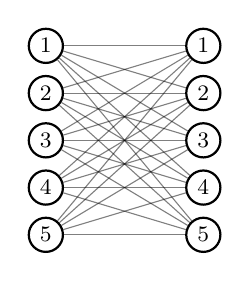
\begin{tikzpicture}
      \tikzstyle{every node} = [draw, circle, thick, inner sep = 2pt]
      \foreach \y in {0,...,4}{
        \pgfmathtruncatemacro{\yplusone}{5 - \y}
        \node(a\y) at (0,.6*\y) {\footnotesize\yplusone};
      }
      \foreach \y in {0,...,4}{
        \pgfmathtruncatemacro{\yplusone}{5 - \y}
        \node(\y) at (2,.6*\y) {\footnotesize\yplusone};
      }

      \foreach \x in {0,...,4}{
        \foreach \y in {0,...,4}{
          \path[opacity=0.5] (a\x) edge (\y);
        }
      }
    \end{tikzpicture}
  \end{center}
  \caption{Examples}
  \label{con_ex}
\end{figure}

\todo{Figure~\ref{con_ex}. It's just a placeholder right now}


Connectivity graphs also allow to graphically modelize how weights are tied in a neural layer. Let's suppose the $\Theta_ij$ are taking their values only into the finite set $K = \{w_1, w_2, \ldots, w_\kappa\}$ of size $\kappa$, which we will refer to as the \emph{kernel} of \emph{weights}. Then we can define a labelling of the edges $s: E \rightarrow K$. $s$ is called the \emph{weight sharing scheme} of the layer. This layer can then be formulated as $\displaystyle \forall v \in M, y_v = \sum_{u \in N, (u,v) \in E} w_{s(u,v)} x_u$. Figure~\ref{cnn} depicts the connectivity graph of a 1-d convolution layer and its weight sharing scheme.

\begin{figure}[h]
  \begin{center}
    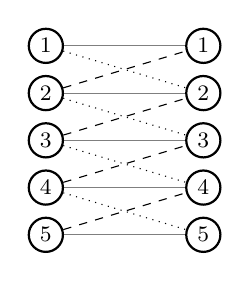
\begin{tikzpicture}
      \tikzstyle{every node} = [draw, circle, thick, inner sep = 2pt]
      \foreach \y in {0,...,4}{
        \pgfmathtruncatemacro{\yplusone}{5 - \y}
        \node(a\y) at (0,.6*\y) {\footnotesize\yplusone};
      }
      \foreach \y in {0,...,4}{
        \pgfmathtruncatemacro{\yplusone}{5 - \y}
        \node(\y) at (2,.6*\y) {\footnotesize\yplusone};
      }
      \path[opacity=0.5]
      (a0) edge (0);
      \path[dashed]
      (a0) edge (1);
      \path[dotted]
      (a1) edge (0);
      \path[opacity=0.5]
      (a1) edge (1);
      \path[dashed]
      (a1) edge (2);
      \path[dotted]
      (a2) edge (1);
      \path[opacity=0.5]
      (a2) edge (2);
      \path[dashed]
      (a2) edge (3);
      \path[dotted]
      (a3) edge (2);
      \path[opacity=0.5]
      (a3) edge (3);
      \path[dashed]
      (a3) edge (4);
      \path[dotted]
      (a4) edge (3);
      \path[opacity=0.5]
      (a4) edge (4);
    \end{tikzpicture}
  \end{center}
  \caption{Depiction of a 1D-convolutional layer and its weight sharing scheme.}
  \label{cnn}
\end{figure}


\todo{Add weight sharing scheme in Figure~\ref{cnn}}

\subsubsection{Computation graph}
\label{comp_graph}

\subsubsection{Underlying graph structure}
\label{inductive_graph}

\subsubsection{Graph-structured dataset}
\label{transductive_graph}

transductive vs inductive

\subsection{Geometric grids}

\subsection{Grid graphs}

\subsection{Spatial graphs}

\subsection{Projections of spatial graphs}

\end{document}